\iffalse
\jk{[\S5.1] The ELBO/KL decomposition seems to take a KL against an \emph{unnormalized} quantity over $U$ (via $\rho^{\theta,\pi}_0$). It may read more cleanly (and be formally correct) if rewritten using the standard identity with a normalized posterior, e.g., $\mathrm{KL}(w(U)\,\|\,p(U\mid x_0))$.}


\jk{[Alg.~1--2 vs. main text] The algorithms use $p^\theta_{t_k}(\cdot\mid x_k)$ / $p^\theta_{t_k}(x_{k-1}\mid x_k)$ notation, while earlier sections use reverse transitions like $p^\theta_{t_{k-1}\mid t_k}(\cdot\mid x_k)$ (and sometimes drop subscripts). Could you standardize the time/conditioning notation so it is unambiguous what distribution is being sampled/evaluated in the algorithms?}

\jk{The text restricts policies to size-$N$ subsets but the §5.2 parameterization samples each index independently with probability $p_i$, so the variable set size should be reconciled with the earlier definition.}

\jk{Calling the independent include/exclude construction a “multinomial distribution over index sets” is misleading unless you enforce an exactly-$N$ draw without replacement.}

\jk{In Algorithm~1 the product term using $\pi_\phi(U_{k-1}\mid x_k)$ looks potentially off by one depending on the convention and it is worth double-checking the indexing.}

\jk{Algorithm~2’s initialization $U_K\leftarrow[L]$ and the $\Delta_k$ update suggest nested “still-masked” sets, while §3.1 says $\{U_1,\dots,U_K\}$ form a partition, so it would help to clarify whether $U_k$ denotes newly unmasked indices or remaining masked indices.}

\fi

\section{Introduction}

\begin{figure}[t]
    \centering
    \begin{subfigure}[t]{0.3\linewidth}
        \centering
        \begin{minipage}[c][0.17\textheight][c]{\linewidth}
            \centering
            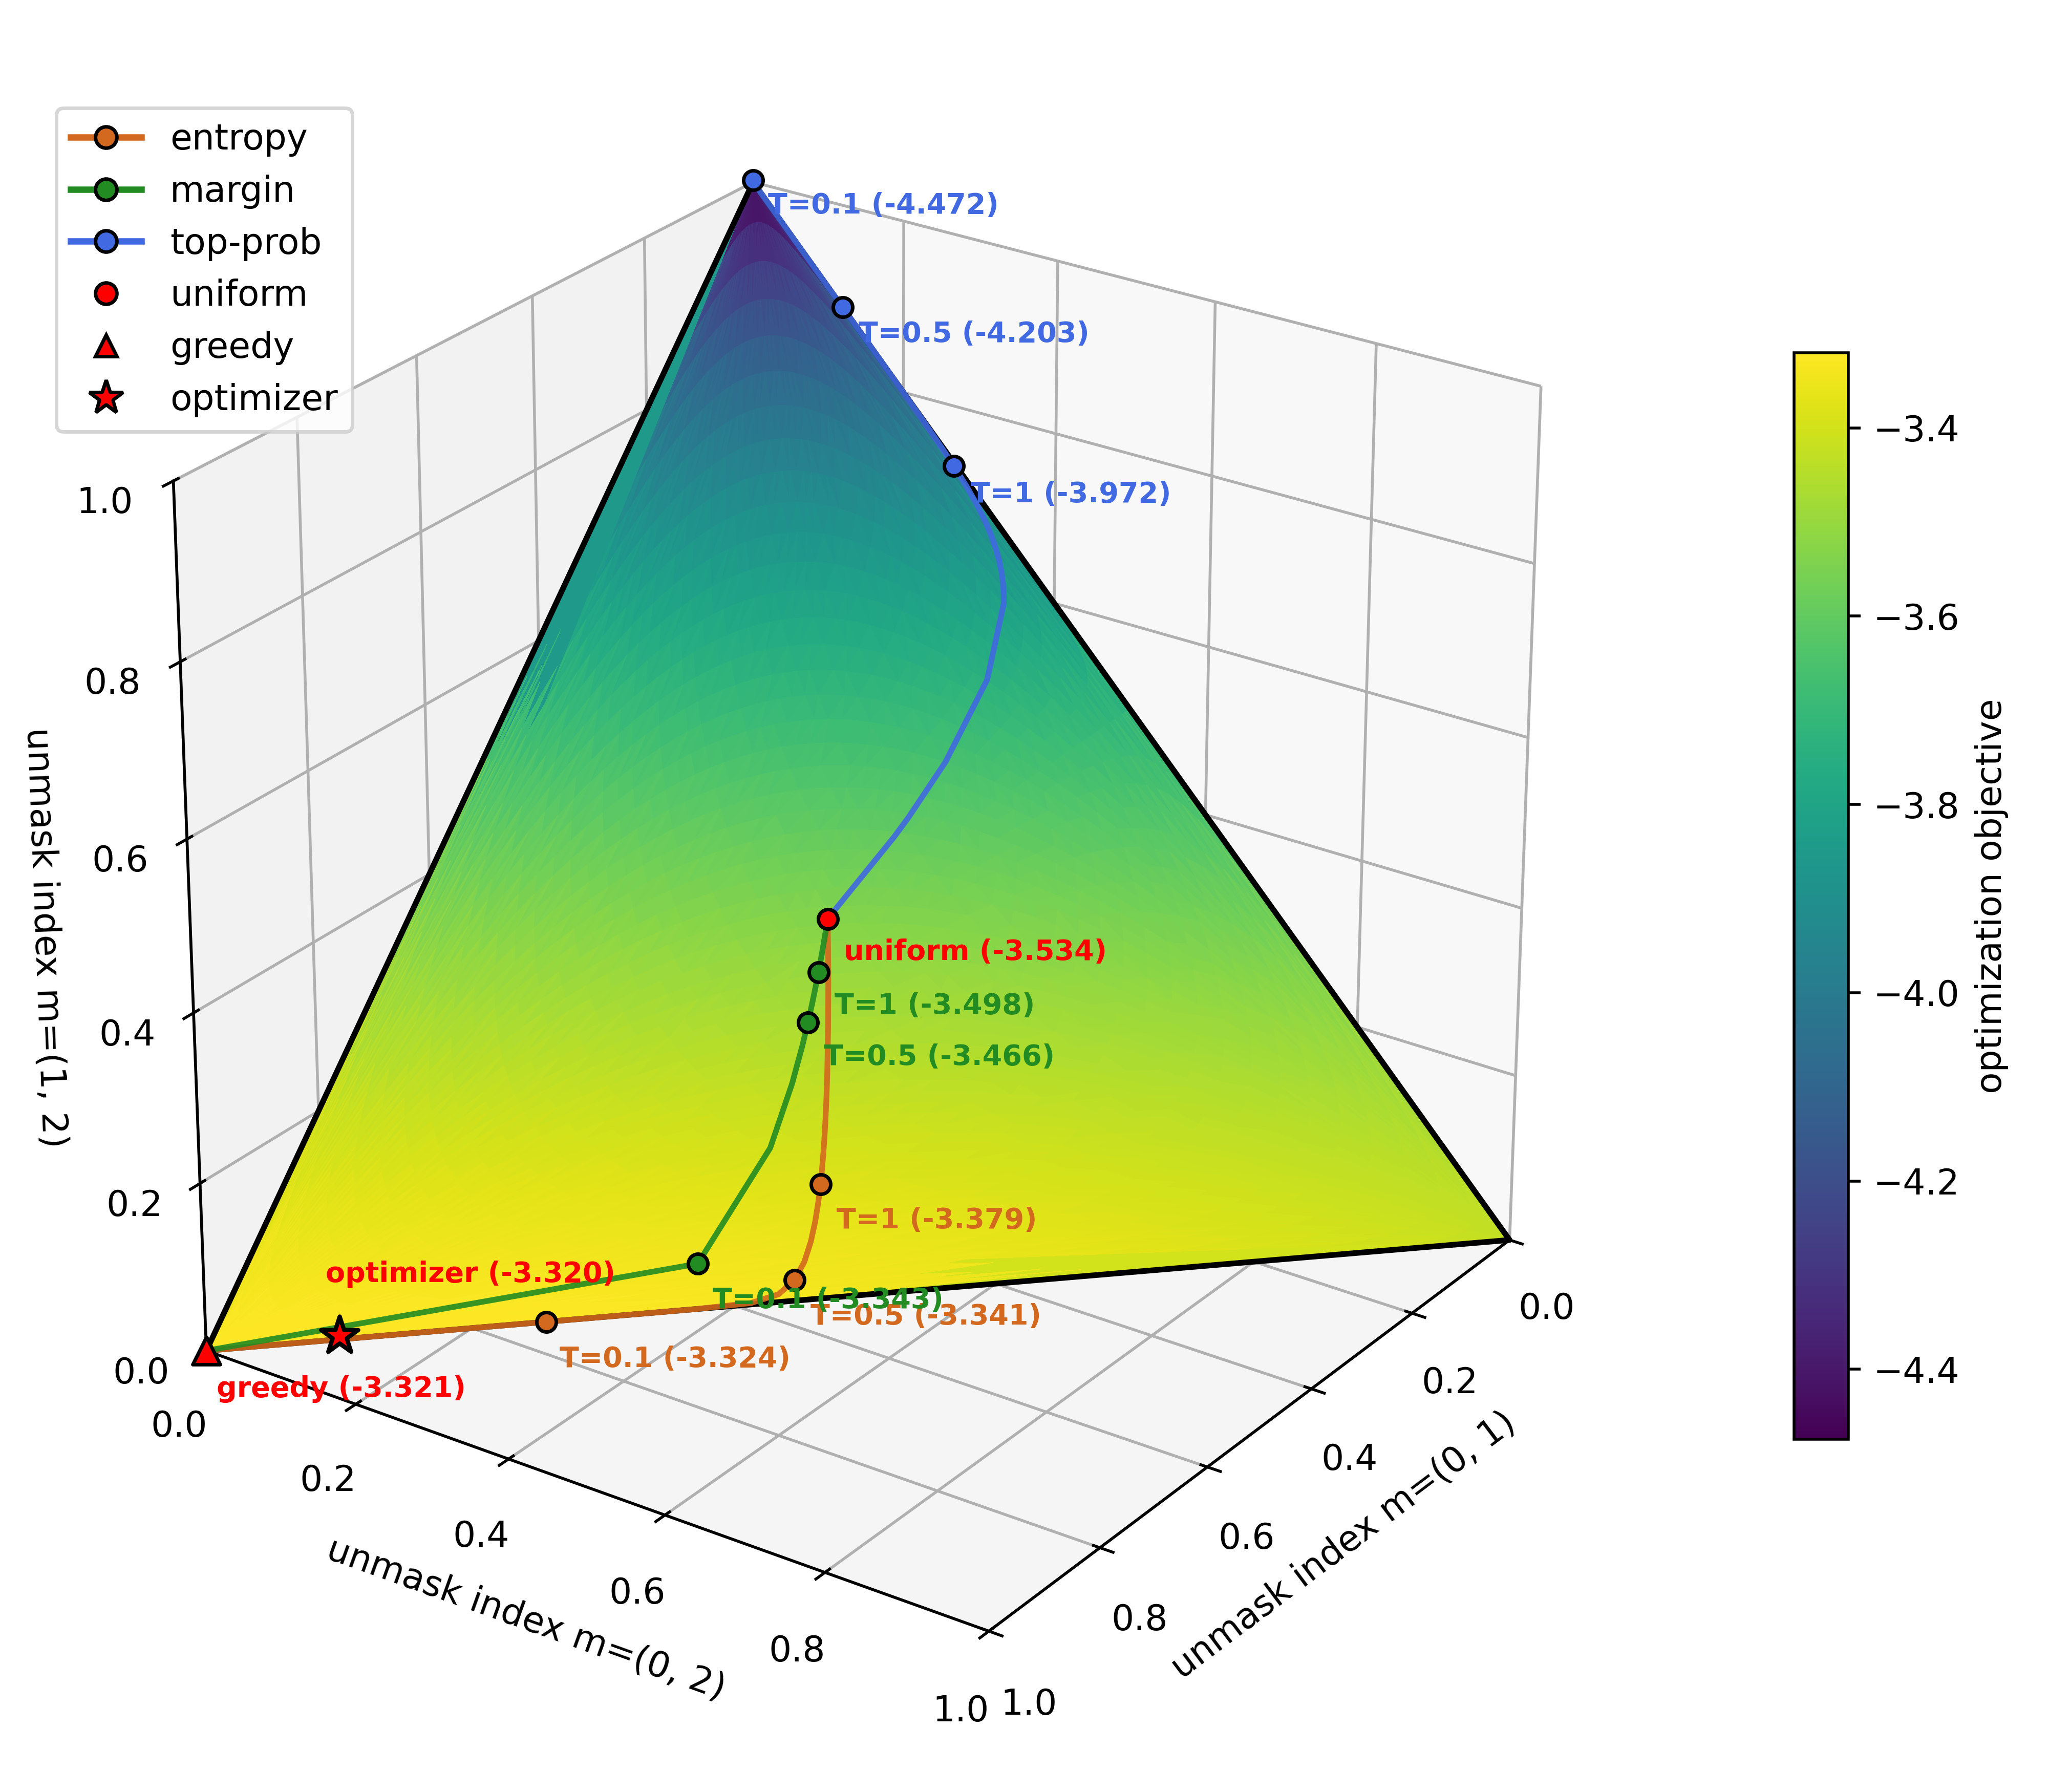
\includegraphics[height=0.17\textheight,width=\linewidth,keepaspectratio]{figs/policy_simplex.png}
        \end{minipage}
        \caption{Landscape on policy simplex.}
        \label{fig:opt-intro}
    \end{subfigure}
    \hfill
    \begin{subfigure}[t]{0.38\linewidth}
        \centering
        \begin{minipage}[c][0.17\textheight][c]{\linewidth}
            \centering
            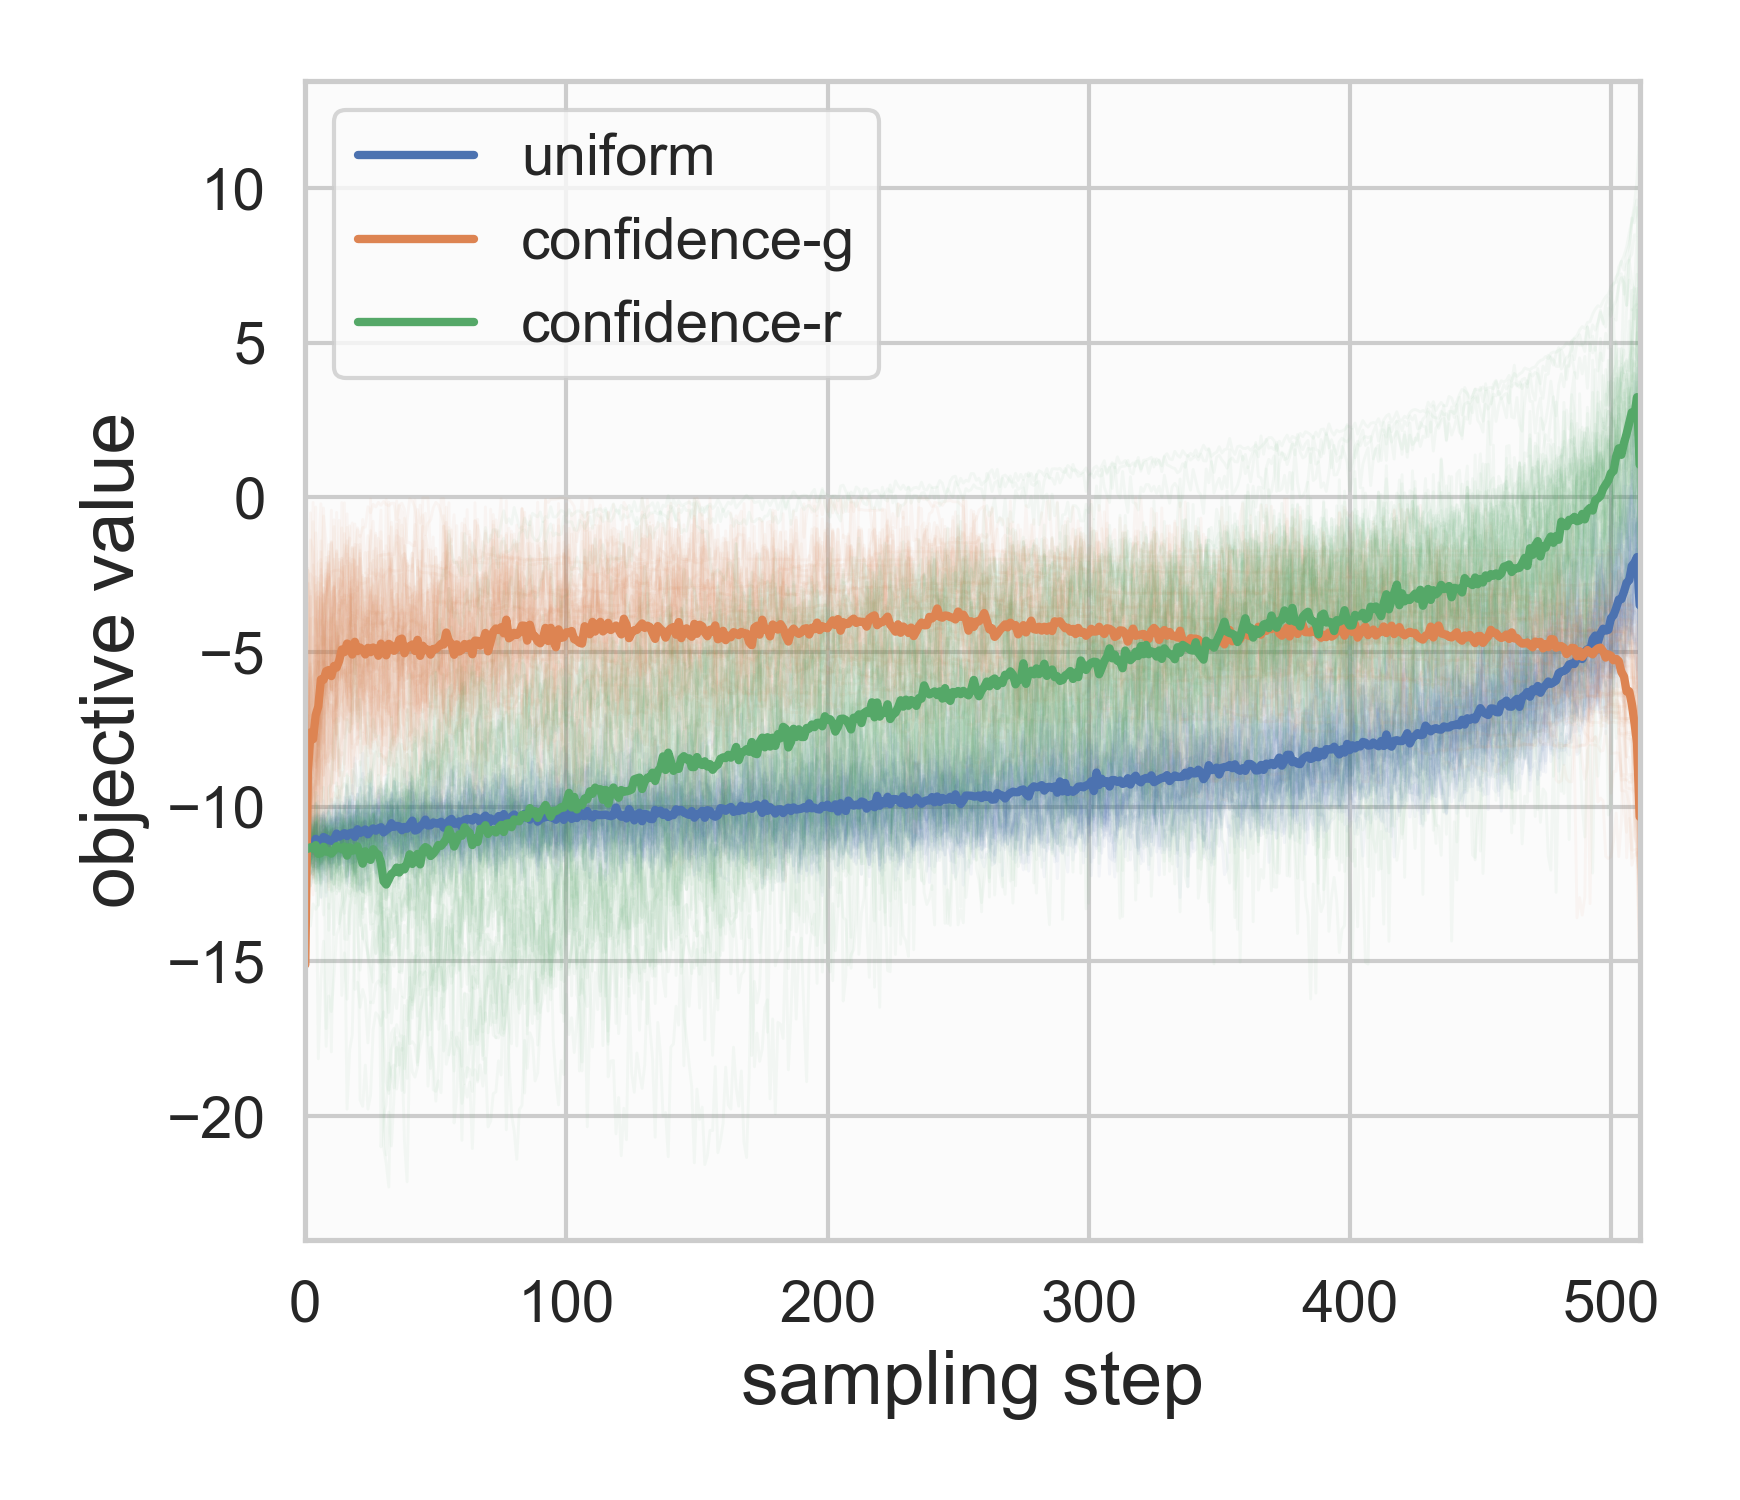
\includegraphics[height=0.17\textheight,width=\linewidth,keepaspectratio]{figs/objective_steps_512.png}
        \end{minipage}
        \caption{Likelihood objectives.}
        \label{fig:radd-obj-val}
    \end{subfigure}
    \hfill
    \begin{subfigure}[t]{0.3\linewidth}
        \centering
        \begin{minipage}[c][0.17\textheight][c]{\linewidth}
            \centering
            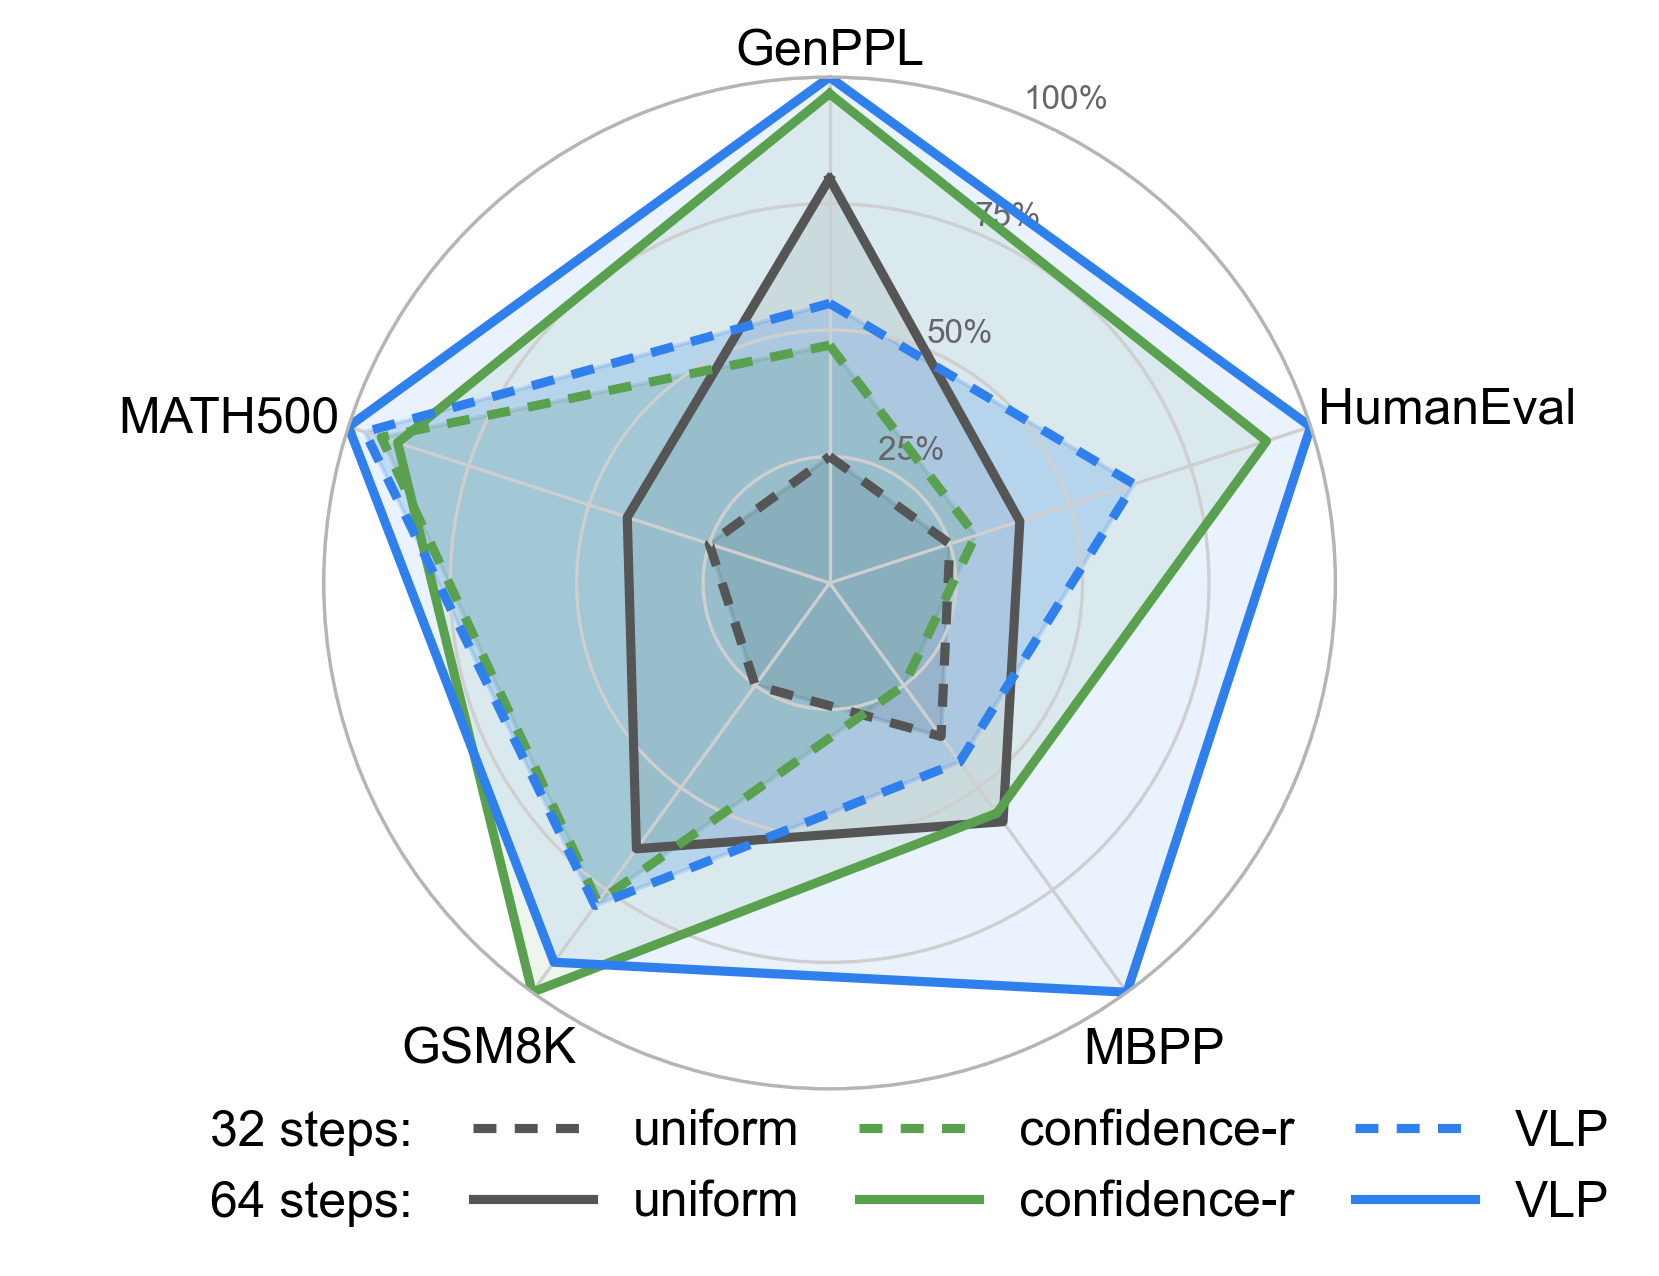
\includegraphics[height=0.17\textheight,width=\linewidth,keepaspectratio]{figs/radar_steps32_64.png}
        \end{minipage}
        \caption{VLP evaluation.}
        \label{fig:vlp-eval}
    \end{subfigure}
    \label{fig:optimality-exp}
    \caption{\textbf{(a)}: The landscape of the local likelihood maximization problem \eqref{eq:trainable_confidence} over the policy simplex, and different unmasking methods with their attained objective values. \textbf{(b)}: Monte Carlo estimation of per-step local objective values \eqref{eq:trainable_confidence} attained by different unmasking methods in text generation with RADD~\citep{ou2025absorbingdiscretediffusionsecretly}. \textbf{(c)}: Selected evaluation results (see Table~\ref{tab:text-gen} and~\ref{tab:dream-all} for full version) of our likelihood-trained policy, VLP, compared to uniform and confidence unmasking methods in RADD text generation, and Dream-7B~\citep{ye2025dream7bdiffusionlarge} code and math generation. Data are rescaled between the best and worst performance among the compared methods.}
\end{figure}

Diffusion language models \citep{li2022diffusion} recently emerged as a potential alternative to their autoregressive counterparts for language modeling with advances in discrete diffusion \citep{austin2021structured, lou2024discrete, sahoo2024simple, shi2024simplified, ou2024your}. These models conduct training and inference by leveraging a forward-backward pair of continuous-time Markov chains (CTMC) evolving over continuous time $t\in(0,1)$ in a discrete state space. In the forward (noising) process, a training data sample is gradually corrupted into pure noise; then the model aims to learn its reverse, i.e. the backward (denoising) process, that refines a random draw from pure noise step by step back to data.

The CTMCs become more specific when we focus on masked diffusion models (MDMs) \citep{shi2024simplified,sahoo2024simple}, currently one of the most representative discrete diffusion schemes for language modeling. In the forward process of MDMs, each token in the input sequence independently jumps to a special mask token \mask{} with the same probability, and stays in \mask{} thereafter. During inference, the backward process begins with an all-mask sequence and learns to perform random unmasking, converting each \mask{} to a predicted text token. In this way, compared to autoregressive models that maintain a left-to-right ordering, MDMs offer an enhanced flexibility in training and generation order.

Nonetheless, sampling from the backward process introduces several practical subtleties. For fast sampling, it is desirable to take large time steps $\Delta t$, unmasking multiple tokens per step. However, the ideal continuous-time process requires $\Delta t \to 0$ to guarantee simulation accuracy. Therefore, as unmasking can be conducted in arbitrary order, which token(s) should we choose to unmask?

Standard MDM training does not answer this question because it only learns a continuous-time transition rate, but several proposals exist. A first idea is to assign each token the same chance of being unmasked at each sampling step, known as $\tau$-leaping strategy \citep{campbell2022continuous} or \textit{uniform} unmasking. The motivation for this approach is that in the continuous-time limit, each token position has the same unmasking rate, symmetric to the forward process. However, this method 
%is not theoretically grounded because the uniform property no longer holds after discretization. As a result, it 
%\jiaxin{I believe the theoretical backward is indeed a uniform choice even under discretization.}
usually underperforms in empirical studies of MDM inference \citep{zhao2024informed}.

\begin{wrapfigure}{r}{0.45\textwidth}
    \vspace{-1em}
    \centering
    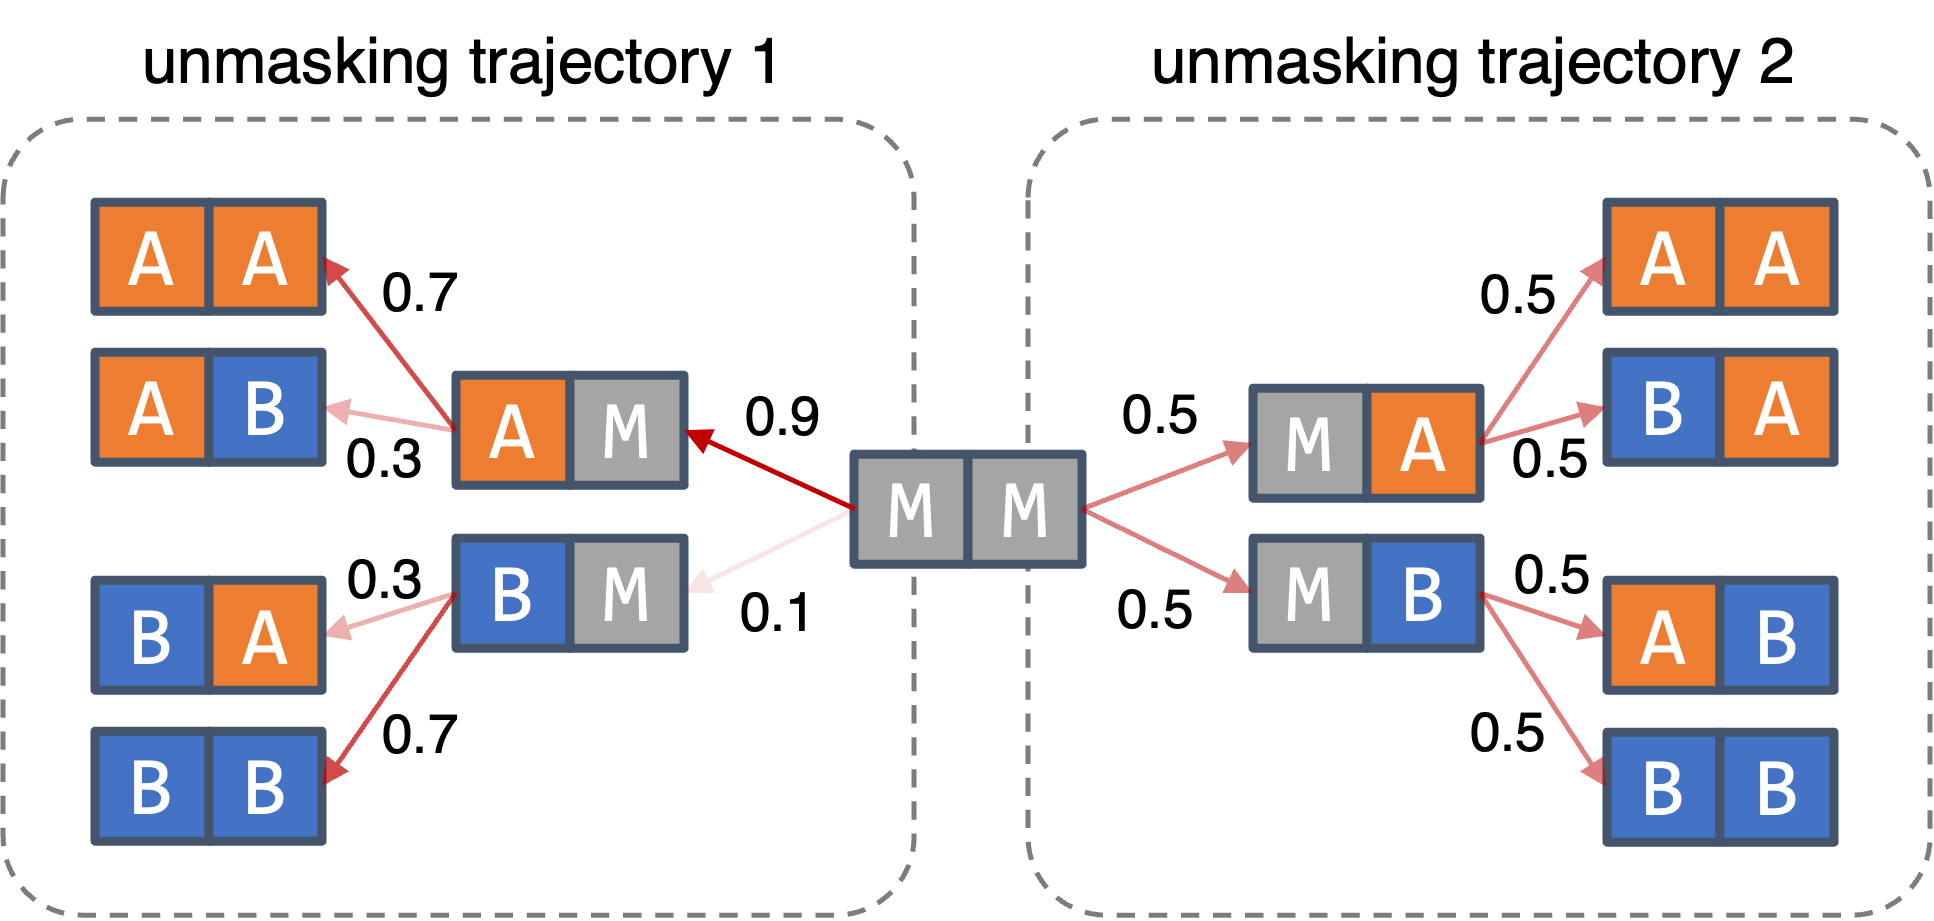
\includegraphics[width=0.98\linewidth]{figs/illustration-icml.png}
    \caption{Two different sampling trajectories of decoding a length-2 sequence on a simple vocabulary $\{\texttt{A},\texttt{B}\}$. Confidence-based unmasking indicates that trajectory 1 is preferred.}
    \label{fig:illustrate}
    \vspace{-1.5em}
\end{wrapfigure}

Another method that works better in practice is \textit{confidence}-based unmasking \citep{kim2025train,nie2025largelanguagediffusionmodels,ye2025dream7bdiffusionlarge}. Specifically, it prioritizes unmasking positions where the model is more confident in its vocabulary distribution. For example, in Figure~\ref{fig:illustrate}, the left masked token has prediction $p(\texttt{A})=0.9,p(\texttt{B})=0.1$, which shows the model's higher confidence than the right position with $p(\texttt{A})=p(\texttt{B})=0.5$, and hence gets unmasked first. Here, confidence can be quantified by various metrics such as negative entropy, top probability, and the margin between the top-2 probabilities; see details in Section~\ref{sec:prelim}.

\subsection{Theoretical Understanding of Confidence}

Despite its empirical success, the design of confidence-based methods remains largely heuristic and the reasons for their success are not fully clear. Although earlier work provides some intuition that these methods plan for a good reasoning path \citep{kim2025train}, there is still a lack of theoretical justification for their advantages over the uniform scheme. This is the first question we aim to address in this paper: \emph{Is confidence unmasking provably better for the time-discretized backward process?}

In the first half of this paper, we formulate an optimization problem of searching for the best unmasking policy $\pi$, that is, the random mapping from current sampling step to the index set for next unmasking step. The objective of the problem is to maximize the sampling log-likelihood $\log p_0^{\theta,\pi}$ with respect to the discrete-time policy $\pi$ and a parameterized backward process $p_t^\theta$ learned separately, i.e.
\begin{align}\label{eq:obj}
    \max_\pi \EE_{\bm x_0\sim q_0}\log p^{\theta,\pi}_0(\bm x_0),
\end{align}
where $q_0$ is the unknown source data distribution. We show that, under a data-agnostic approximation and a local restriction of objective for tractability, entropy-based confidence unmasking emerges as a (near-)optimal policy (Section~\ref{sec:confidence}). This indicates a provable advantage of confidence unmasking over other methods in terms of sample likelihood, consistent with empirical observations. We also conduct numerical evaluations in synthetic and real text generation tasks to support our theoretical claims on the near-optimality of confidence-based unmasking methods (Figure~\ref{fig:opt-intro},~\ref{fig:radd-obj-val}).

\subsection{Unmasking Policy via Likelihood Optimization}
On the other hand, the reductions in our theory also suggest that confidence unmasking is not optimal, as it does not maximize the original objective \eqref{eq:obj}. This motivates us to revisit \eqref{eq:obj} and ask a second question: \emph{Can we further develop advanced unmasking policies based on the original likelihood optimization problem?}

The second half of this paper is devoted to this extension from confidence to trainable policies. Specifically, we develop Variational Likelihood Policy (\alg{}), a prototypical training framework based on \eqref{eq:obj} with variational inference to optimize a neural-network-parameterized policy $\pi$, serving as an auxiliary trainable component to pretrained MDMs (Section~\ref{sec:method}). We train and evaluate \alg{} on differently scaled DLMs, including RADD~\citep{ou2025absorbingdiscretediffusionsecretly}, Dream-7B~\citep{ye2025dream7bdiffusionlarge}, and DiffuCoder-7B~\citep{gong2025diffucoderunderstandingimprovingmasked} across text, code, and math generation tasks (Figure~\ref{fig:vlp-eval}). The evaluation results indicate that our likelihood-trained policy, \alg{}, effectively learns unmasking policies and consistently matches or surpasses the performance of confidence-based methods across different models and tasks.

To summarize, in this paper, we propose a systematic framework based on likelihood optimization to analyze MDM unmasking methods. Our contribution lies in

\begin{itemize}[noitemsep, topsep=0pt]
    \item \textbf{Theoretical understanding of confidence:} We prove the theoretical advantages of confidence unmasking in terms of near-optimality in likelihood optimization (Section~\ref{sec:confidence}), supported by numerical analysis on the optimization objective in synthetic and real generation scenarios (Section~\ref{subsec:numerical-analysis}; Figure~\ref{fig:opt-intro},~\ref{fig:radd-obj-val}).

    \item \textbf{Principled design of trainable unmasking methods:} We design a likelihood-trained unmasking policy, \alg{} (Section~\ref{sec:method}), with variational inference and show its advantages through comprehensive evaluations across text, code, and math generation tasks on MDMs at different scales (Section~\ref{subsec:vlp-eval}; Figure~\ref{fig:vlp-eval}).

\end{itemize}